\documentclass[letterpaper,12pt,fleqn]{article}
\usepackage{matharticle}
\usepackage{tikz}
\usetikzlibrary{positioning}
\pagestyle{empty}
\begin{document}
\section*{Cardinality}

\begin{definition}[Cardinality]
  To say that two sets \(A\) and \(B\) have the same \emph{cardinality}, denoted by \(\abs{A}=\abs{B}\), means that
  there exists a bijection \(f:A\to B\).
\end{definition}

\begin{notation}
  Let \(n\in\N\):
  \[[n]=\set{1,\ldots,n}\]
\end{notation}

\begin{definition}[Finite]
  To say that a set \(A\) is \emph{finite} means that either \(A=\emptyset\) or there exists a bijection
  \(f:A\to[n]\) for some \(n\in\N\).  For the empty set: \(\abs{\emptyset}=0\).  For a non-empty finite set:
  \(\abs{A}=n\).  If \(A\) is not finite then it is \emph{infinite}.
\end{definition}

\begin{definition}[Countable]
  To say that a set \(A\) is \emph{countable} means that either \(A\) is finite or \(\abs{A}=\abs{\N}\).  If \(A\)
  is not countable then it is \emph{uncountable}.
\end{definition}

\begin{theorem}
  \(\abs{\Z}=\abs{\N}\)
\end{theorem}

\begin{proof}
  Let \(f:\N\to\Z\) be the bijection that enumerates the elements in \(\Z\) as follows:
  \begin{align*}
    f(1) &= 0 \\
    f(2) &= -1 \\
    f(3) &= 1 \\
    f(4) &= -2 \\
    f(5) &= 2 \\
    \vdots
  \end{align*}
  Therefore \(\abs{\Z}=\abs{\N}\).
\end{proof}

\begin{theorem}
  \(\abs{2\N}=\abs{\N}\)
\end{theorem}

\begin{proof}
  Let \(f:\N\to2\N\) be the bijection that enumerates the elements in \(2\N\) as follows:
  \begin{align*}
    f(1) &= 2 \\
    f(2) &= 4 \\
    f(3) &= 6 \\
    f(4) &= 8 \\
    f(5) &= 10 \\
    \vdots
  \end{align*}
  Therefore \(\abs{2\N}=\abs{\N}\).
\end{proof}

\begin{theorem}
  Every subset of \(N\) is countable.
\end{theorem}

\begin{proof}
  Assume \(U\subset\N\).  If \(U\) is finite then done, so assume that \(U\) is infinite.  By the well-ordering
  principle, there exists some least element \(u_1\in U\) and \(U=\set{u_1,u_2,u_3,\ldots}\) can be ordered such
  that \(u_1<u_2<u_3<\cdots\).  So let \(f:\N\to U\) be defined by \(f(i)=u_i\).  Thus, \(f\) is a bijection that
  enumerates the elements in \(U\).

  Therefore \(U\) is countable.
\end{proof}

\begin{corollary}
  Let \(A\) and \(B\) be sets such that \(A\subset B\).  If \(B\) is countable then \(A\) is countable.
\end{corollary}

\begin{proof}
  Assume that \(B\) is countable.  If \(B\) is finite then \(A\) must be finite and thus countable, so assume that
  \(B\) is infinite.  This means that there exists a bijection \(f:B\to\N\), and so \(f_A:A\to\N\) must be a
  bijection to a subset of \(N\).  But all subsets of \(N\) are countable.

  Therefore \(A\) is countable.
\end{proof}

\begin{corollary}
  Let \(A\) and \(B\) be sets such that \(A\subset B\).  If \(A\) is uncountable then \(B\) is uncountable.
\end{corollary}

\begin{theorem}
  Every infinite set has a countably infinite subset.
\end{theorem}

\begin{proof}
  Assume that \(X\) is an infinite set.  If \(X\) is countable then done, so assume that \(X\) is uncountable.
  Select \(x_1\in X\) and let \(U=\set{x_1,x_2,x_3,\ldots}\) where \(x_i\in X\) and \(x_{i+1}\) is selected from
  \(X-\left(\bigcup_{j=1}^i\set{x_j}\right)\).  Now, let \(f:\N\to U\) be defined by \(f(i)=u_i\).  Thus, \(f\) is a
  bijection that enumerates the elements in \(U\).

  Therefore \(U\subset X\) and \(U\) is countable.
\end{proof}

\begin{theorem}
  A set if finite if and only if every injection on the set is bijective.
\end{theorem}

\begin{proof}
  Let \(X\) be a set.  \(X\) is finite iff for every injection \(f:X\to X\) it is the case that
  \(\abs{f(X)}=\abs{X}\) iff every injection on \(X\) is bijective.
\end{proof}

\begin{theorem}
  A set is infinite if and only if there exists an injection from the set to a proper subset of itself.
\end{theorem}

\begin{proof}
  \(X\) is finite if and only if every injection on \(X\) is bijective, is equivalent to:
  \(X\) is infinite if and only if there exists an injection on \(X\) that is not bijective, is equivalent to:
  \(X\) is infinite if and only if there exists an injection on \(X\) that is not surjective, is equivalent to:
  \(X\) is infinite if and only if there exists an injection on \(X\) to a proper subset of itself.
\end{proof}

\begin{example}
  If \(X\) is infinitely countable then all infinite subsets are also countable, so assume that \(X\) is uncountable.
  An injection to a proper subset can be constructed as follows:
  \begin{enumerate}
  \item Select an infinitely countable subset of \(X\) and call it \(U\).
  \item Construct an infinitely countable subset of \(U\) and call it \(S\).  Note that \(\abs{S}=\abs{U}\).
  \item Select a bijection \(g:U\to S\).
  \item Construct the set \(A=S\cup(X-U)\).  Note \(A\subsetneq X\), since it does not contain the elements in
    \(U-S\).
  \item Define the injection \(f:X\to A\) as follows:
    \[f(x)=\begin{cases}
    g(x), & x\in U \\
    x, & x\notin U
    \end{cases}\]
  \end{enumerate}
\end{example}

\begin{theorem}
  The union of two countable sets is countable.
\end{theorem}

\begin{proof}
  Let \(A\) and \(B\) be two countable sets.  Since it is possible that \(A\cap B\ne\emptyset\) define new sets as
  follows:
  \begin{align*}
    A' &= A \\
    B' &= B-A
  \end{align*}
  Note that \(A\cup B=A'\cup B'\) and \(A'\cap B'=\emptyset\).  If \(A'\) or \(B'\) is finite then the finite
  set(s) can be enumerated first, followed by any countably infinite set, so assume that neither \(A'\) nor \(B'\)
  are finite.  Let \(A'=\set{a_1,a_2,\ldots}\) and \(B'=\set{b_1,b_2,\ldots}\) and define \(f:\N\to A'\cup B'\) as
  follows:
  \begin{align*}
    f(1) &= a_1 \\
    f(2) &= b_1 \\
    f(3) &= a_2 \\
    f(4) &= b_2 \\
    \vdots
  \end{align*}
  Thus, \(f\) is a bijection that enumerates the elements of \(A'\cup B'\) and hence \(A'\cup B'\) is countable.

  \(\therefore A\cup B\) is countable.
\end{proof}

\begin{lemma}
  Let \(\set{U_i:i\in N}\) be a countably infinite number of countably infinite sets such that the \(U_i\) are
  pairwise disjoint.  Then:
  \[U=\bigcup_{i\in\N}U_i\]
  is countable.
\end{lemma}

\begin{proof}
  Let \(U_i=\set{u_{ij}:j\in\N}\) and arrange the \(U_i\) as the rows of a matrix.  Note that the \(u_{ij}\) are
  distinct and in one-to-one correspondence with the elements of \(U\).

  Now, enumerate the \(u_{ij}\) along the diagonals as follows:

  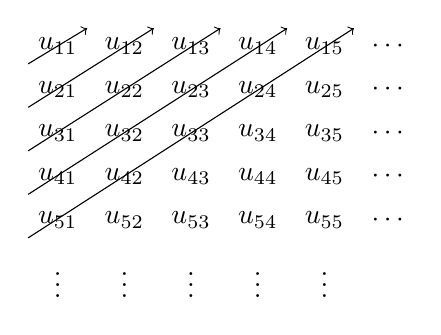
\begin{tikzpicture}[node distance=0.1cm]
    \node (u11) at (0,0) {\(u_{11}\)};
    \node (u12) [right=of u11] {\(u_{12}\)};
    \node (u13) [right=of u12] {\(u_{13}\)};
    \node (u14) [right=of u13] {\(u_{14}\)};
    \node (u15) [right=of u14] {\(u_{15}\)};
    \node (u1n) [right=of u15] {\(\cdots\)};
    \node (u21) [below=of u11] {\(u_{21}\)};
    \node (u22) [below=of u12] {\(u_{22}\)};
    \node (u23) [below=of u13] {\(u_{23}\)};
    \node (u24) [below=of u14] {\(u_{24}\)};
    \node (u25) [below=of u15] {\(u_{25}\)};
    \node (u2n) [right=of u25] {\(\cdots\)};
    \node (u31) [below=of u21] {\(u_{31}\)};
    \node (u32) [below=of u22] {\(u_{32}\)};
    \node (u33) [below=of u23] {\(u_{33}\)};
    \node (u34) [below=of u24] {\(u_{34}\)};
    \node (u35) [below=of u25] {\(u_{35}\)};
    \node (u3n) [right=of u35] {\(\cdots\)};
    \node (u41) [below=of u31] {\(u_{41}\)};
    \node (u42) [below=of u32] {\(u_{42}\)};
    \node (u43) [below=of u33] {\(u_{43}\)};
    \node (u44) [below=of u34] {\(u_{44}\)};
    \node (u45) [below=of u35] {\(u_{45}\)};
    \node (u4n) [right=of u45] {\(\cdots\)};
    \node (u51) [below=of u41] {\(u_{51}\)};
    \node (u52) [below=of u42] {\(u_{52}\)};
    \node (u53) [below=of u43] {\(u_{53}\)};
    \node (u54) [below=of u44] {\(u_{54}\)};
    \node (u55) [below=of u45] {\(u_{55}\)};
    \node (u5n) [right=of u55] {\(\cdots\)};
    \node (um1) [below=of u51] {\(\vdots\)};
    \node (um2) [below=of u52] {\(\vdots\)};
    \node (um3) [below=of u53] {\(\vdots\)};
    \node (um4) [below=of u54] {\(\vdots\)};
    \node (um5) [below=of u55] {\(\vdots\)};
    \draw [->] (u11.south west) -- (u11.north east);
    \draw [->] (u21.south west) -- (u12.north east);
    \draw [->] (u31.south west) -- (u13.north east);
    \draw [->] (u41.south west) -- (u14.north east);
    \draw [->] (u51.south west) -- (u15.north east);
  \end{tikzpicture}

  This is a one-to-one correspondence between the \(u_{ij}\) and \(\N\) and hence the \(u_{ij}\) are countable.

  Therefore, \(U\) is countable.
\end{proof}

\begin{theorem}
  The union of countably many countable sets is countable.
\end{theorem}

\begin{proof}
  Let \(A=\bigcup_{i\in I}A_i\) be a union of countably many countable sets.  In order to remove duplicates from the
  \(A_i\) (elements in the intersections of two or more \(A_i\)), let:
  \begin{align*}
    A_1' &= A_1 \\
    A_i' &= A_i-\bigcup_{j=1}^{i-1}A_j
  \end{align*}
  Note that the \(A_i'\) are pairwise disjoint and \(A=\bigcup_{i\in I}A_i'\)

  Now arrange the \(A_i'\) as the rows of a matrix \(B\).  This means that the \(b_{ij}\) are distinct and in
  one-to-one correspondence with the elements of \(A\).  Let \(U\) be a matrix consisting of a countably infinite
  number of rows and columns as described in the preceding lemma.  There is an injection between the rows in \(B\)
  and the rows in \(U\).  Furthermore, there is an injection between the columns of each row \(B_i\) and its
  corresponding row \(U_i\).  Thus, there is a one-to-one correspondence between the elements of \(B\), and hence
  the elements of \(A\), and the elements of some subset \(C\) of the elements of \(U\).  But the subset of a
  countable set is countable and so \(C\) is countable.

  Therefore \(A\) is countable.
\end{proof}

\begin{theorem}
  The set \(\Q\) is countable.
\end{theorem}

\begin{proof}
  Let \(\set{Q_i:i\in\N}\) be a family of sets where \(Q_i=\setb{\frac{p}{i}}{p\in\Z}\).  Note that:
  \[\Q=\bigcup_{i\in\N}Q_i\]
  But \(\set{Q_i:i\in\N}\) is a countable number of countable sets, and hence is countable.

  Therefore, \(Q\) is countable.
\end{proof}

\begin{theorem}
  The set of all finite subsets of a countable set is countable.
\end{theorem}

\begin{proof}
  Assume that \(A\) is a countable set.  Let \(A_i\) be the set of all finite subsets of \(A\) such that
  \(\abs{A_i}=i\in\N\) and let \(\set{A_i:i\in\N}\) be the family of all such sets.  Note that
  \(B=\bigcup_{i\in\N}A_i\) is a union of a countable number of finite (countable) sets.

  Therefore, \(B\) is countable.
\end{proof}

\end{document}
